\section{Sound singularities}\label{sec:singularity}

\subsection{Singular chains}

Let the chain of Section~\ref{sec:chains} run forever: step $n\ge1$ costs $g_{n}$ per candidate to generate and $a_{n}$ per run to check, is incorrect with probability $\rho_{n}$, and is checked by $r_{n}$ runs of a sharp check of soundness $\eps$, all steps independent. The total cost is $T_{\infty}=\sum_{n}T_{n}$ and $F$ counts the steps whose kept candidate is incorrect.

\begin{definition}\label{def:singular}
The chain is \emph{singular} if $\EE\,T_{\infty}<\infty$, and \emph{sound} if $F<\infty$ almost surely.
\end{definition}

If cost is time, a singular chain completes infinitely many improvements in finite expected time, which is the vertical asymptote of the explosion literature \cite{Goo66,Ord26}; if cost is compute or energy, it completes them on a finite budget. Soundness asks that only finitely many of the improvements be wrong, so that from some step on the system is correct.

\begin{proof}[Proof of Theorem~\ref{thm:E}]
Put $\gamma=1-\bar\rho$. By Lemma~\ref{lem:onestep}, $g_{n}+a_{n}r_{n}\le\EE\,T_{n}\le(g_{n}+a_{n}r_{n})/\gamma$ and $\rho_{\ast}\eps^{r_{n}}\le\pi_{n}\le\eps^{r_{n}}/\gamma$. So $\EE\,T_{\infty}<\infty$ if and only if $\sum(g_{n}+a_{n}r_{n})<\infty$, and $\sum\pi_{n}<\infty$ if and only if $\sum\eps^{r_{n}}<\infty$.

(i) Let $E_{n}$ be the event that the candidate kept at step $n$ is incorrect, so $F=\sum\ind_{E_{n}}$ and the $E_{n}$ are independent with $\PR(E_{n})=\pi_{n}<1$. If $\sum\pi_{n}<\infty$, then $\EE F<\infty$, so $F<\infty$ almost surely (this is the first Borel--Cantelli lemma \cite{Bor09,Dur19}), and $\PR(F=0)=\prod_{n}(1-\pi_{n})>0$, because a product of factors in $(0,1]$ converges to a positive limit when the sum of the complements converges. If $\sum\pi_{n}=\infty$, the second Borel--Cantelli lemma for independent events gives $\PR(E_{n}\text{ infinitely often})=1$, so $F=\infty$ almost surely and $\PR(F=0)=0$.

(ii) If every $r_{n}\ge1$, then $\sum a_{n}r_{n}\ge\sum a_{n}$, so a singular chain needs $\sum g_{n}<\infty$ and $\sum a_{n}<\infty$; conversely $r_{n}=1$ gives $\EE\,T_{\infty}\le\sum(g_{n}+a_{n})/\gamma<\infty$.

(iii) A sound singular chain needs $\sum g_{n}<\infty$, $\sum a_{n}r_{n}<\infty$ and $\sum\eps^{r_{n}}<\infty$. The last forces $r_{n}\ge1$ for all large $n$, so $\sum a_{n}<\infty$, and Proposition~\ref{prop:integer} (applied to the tail on which $a_{n}\le1$) gives $\sum a_{n}\log(1/a_{n})<\infty$. Conversely, under the three conditions, the schedule $r_{n}=\lceil\log(1/a_{n})/L\rceil$ of Proposition~\ref{prop:integer}, raised to at least one run, has $\sum a_{n}r_{n}<\infty$ and $\sum\eps^{r_{n}}<\infty$.
\end{proof}

The theorem has a simple form: the chain can reach the asymptote if the steps get cheap fast enough, and it can reach it soundly if they get cheap fast enough to pay for the entropy. Since $a\log(1/a)\ge a$ for $a\le1/e$, the second condition is strictly stronger, and the next corollary shows that the gap between them is not empty.

\begin{corollary}[The soundness gap]\label{cor:gap}
Let $a_{n}=1/(n\log^{\beta}n)$ for $n\ge3$, with $\sum g_{n}<\infty$. A singular chain with every step checked exists if and only if $\beta>1$, and a sound singular chain exists if and only if $\beta>2$. For $1<\beta\le2$ every singular chain keeps infinitely many incorrect modifications almost surely.
\end{corollary}

\begin{proof}
The series $\sum1/(n\log^{c}n)$ converges if and only if $c>1$, by Cauchy's condensation test: its terms decrease, and $2^{k}$ times the term at $n=2^{k}$ is $(k\log2)^{-c}$ (Appendix~\ref{app:condensation}). So $\sum a_{n}<\infty$ if and only if $\beta>1$. For the entropy, $\log(1/a_{n})=\log n+\beta\log\log n$, which lies between $\log n$ and $2\log n$ for all large $n$, so $a_{n}\log(1/a_{n})$ lies between $1/(n\log^{\beta-1}n)$ and twice it, and $\sum a_{n}\log(1/a_{n})<\infty$ if and only if $\beta-1>1$. Theorem~\ref{thm:E} concludes; the last claim is part (i), since a singular chain with $1<\beta\le2$ cannot have $\sum\eps^{r_{n}}<\infty$.
\end{proof}

Figure~\ref{fig:price}(b) shows the condensed partial sums of the two series for three values of $\beta$.

\subsection{Power laws}

The case that matters for growth models is a power law, $a_{n}=n^{-p}$ with $p>1$. Then $A=\zeta(p)$, the profile has entropy
\[
H(p)=\log\zeta(p)+p\,\frac{-\zeta'(p)}{\zeta(p)},
\]
by \eqref{eq:AH}, and $\sum a_{n}\log(1/a_{n})=p\sum n^{-p}\log n<\infty$ for every $p>1$. So every power law admits a sound singularity, and the question is its price.

\begin{proposition}[Price of a power-law takeoff]\label{prop:powerlaw}
As $p\to1^{+}$,
\[
\begin{aligned}
H(p)&=\frac1{p-1}+\log\frac1{p-1}+O(1),\\
\frac{\Vs(\theta)}{A}&=\frac1{(p-1)L}+O\Bigl(\log\frac1{p-1}\Bigr),
\end{aligned}
\]
for fixed $\theta\in(0,1]$ and $\eps$, so that $\Vs(\theta)=\frac{1}{(p-1)^{2}L}\bigl(1+O((p-1)\log\frac1{p-1})\bigr)$.
\end{proposition}

\begin{proof}
Put $t=p-1$. Comparing the decreasing function $x^{-p}$ with its integral, $1/t=\int_{1}^{\infty}x^{-p}\,dx\le\zeta(p)\le1+1/t$. The function $f(x)=x^{-p}\log x$ vanishes at $1$, increases on $[1,e^{1/p}]$ and decreases afterwards, with maximum $1/(pe)$, so $\bigl|\sum_{n\ge1}f(n)-\int_{1}^{\infty}f\bigr|\le1/(pe)$ (Appendix~\ref{app:zeta}); and $\int_{1}^{\infty}x^{-p}\log x\,dx=1/t^{2}$. Hence $-\zeta'(p)=1/t^{2}+O(1)$ and
\[
\frac{-p\zeta'(p)}{\zeta(p)}=\frac{(1+t)(t^{-2}+O(1))}{t^{-1}(1+O(t))}=\frac1t+O(1)
\]
and $\log\zeta(p)=\log\frac1t+O(t)$.
This is the first formula. The second follows from Theorem~\ref{thm:A}, Proposition~\ref{prop:infinite} and $A=1/t+O(1)$.
\end{proof}

The constant term is $1-\gamma_{E}$, where $\gamma_{E}$ is Euler's constant, as the Laurent expansion $\zeta(p)=1/t+\gamma_{E}+O(t)$ shows; at $p=1.1$ the three terms give $12.725$ against the exact $H=12.745$. So the cheapest sound takeoff along a power law near the critical exponent costs, per unit of the cost of one run per step, about $1/((p-1)L)$, and in total about $1/((p-1)^{2}L)$: the soundness of the takeoff is paid for with one extra factor $1/(p-1)$ (Fig.~\ref{fig:price}(a)).

\begin{figure*}[t]
\centering
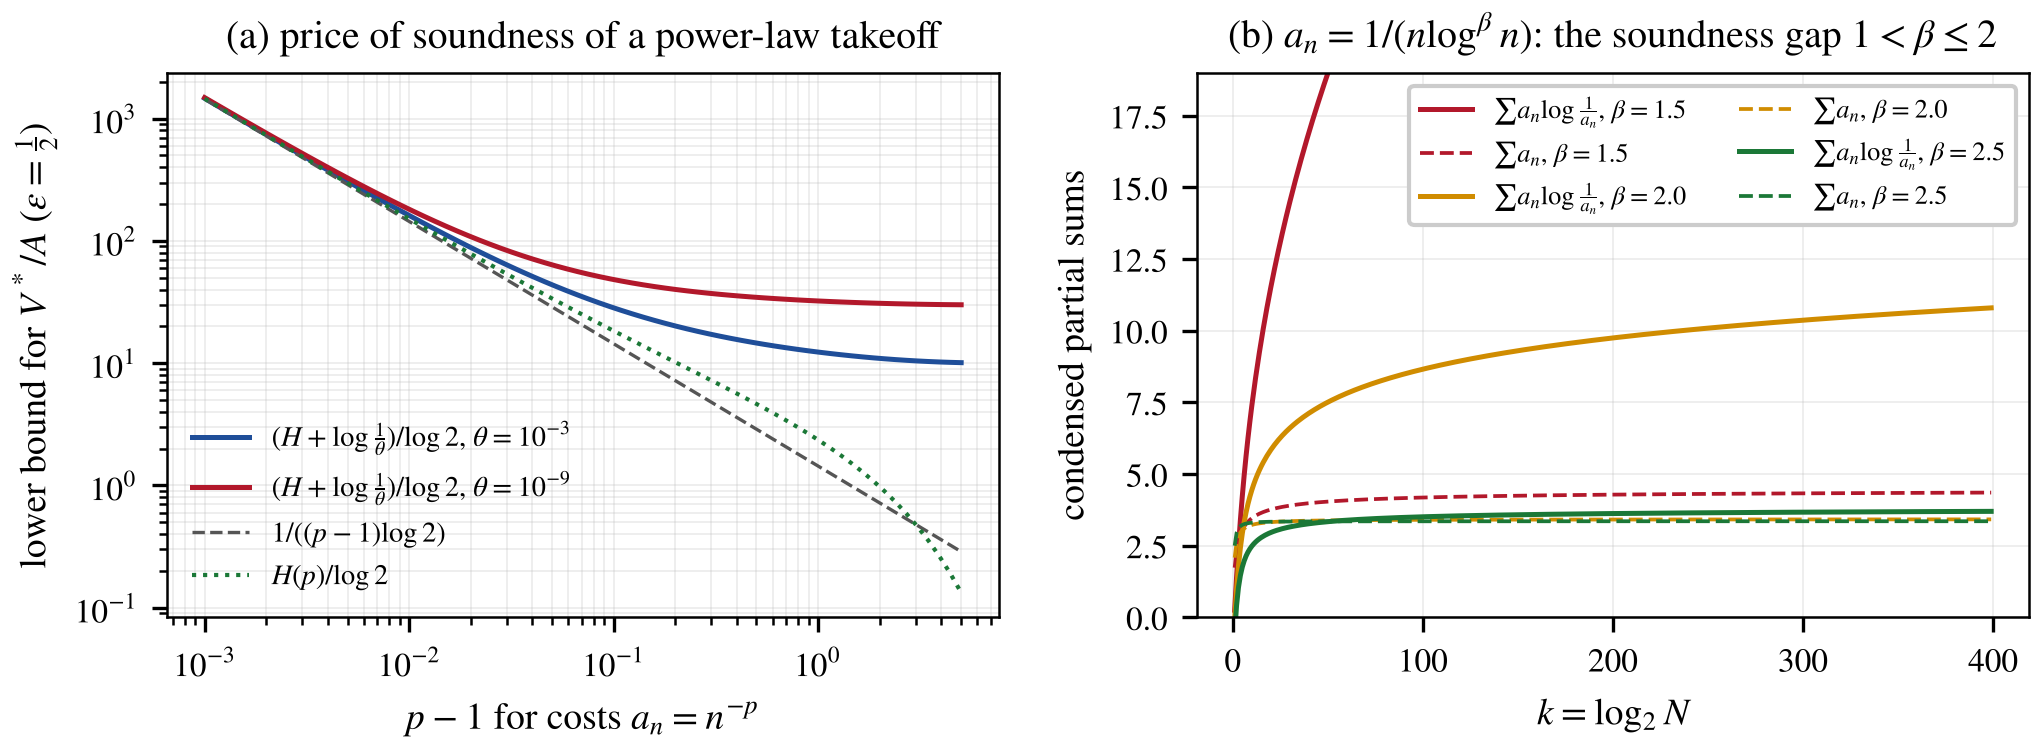
\includegraphics[width=0.98\textwidth]{figures/fig_price}
\caption{(a) The lower bound $(H(p)+\log\frac1\theta)/\log2$ for $\Vs/A$ along the power laws $a_{n}=n^{-p}$, with $\eps=\frac12$ and $\theta=10^{-3}$, $10^{-9}$; as $p\to1$ it approaches $1/((p-1)\log2)$ (dashed), the term that dominates the entropy (dotted). (b) The soundness gap of Corollary~\ref{cor:gap}: condensed partial sums of $\sum a_{n}$ (dashed) and $\sum a_{n}\log\frac1{a_{n}}$ (solid) for $a_{n}=1/(n\log^{\beta}n)$. At $\beta=1.5$ the cost converges and the entropy diverges; at $\beta=2$ the entropy still diverges, like $\log\log N$; at $\beta=2.5$ both converge.}
\label{fig:price}
\end{figure*}

\subsection{Polynomial checks and the phase diagram}

With checks of order $s$, Corollary~\ref{cor:dualcases}(ii) replaces the entropy condition by $\sum a_{n}^{1/(1+s)}<\infty$.

\begin{corollary}[Phase diagram]\label{cor:phase}
Let $a_{n}=n^{-p}$ and $\sum g_{n}<\infty$. A singular chain with every step checked exists if and only if $p>1$. With exponential checks a sound one exists for every $p>1$; with checks of order $s$ a sound one exists if and only if $p>1+s$. For geometric costs $a_{n}=c^{n}$, $0<c<1$, a sound singular chain exists for every $s$.
\end{corollary}

\begin{proof}
The series $\sum n^{-p/(1+s)}$ converges if and only if $p>1+s$, and the series $\sum c^{n/(1+s)}$ converges for every $s$. For the singular part, a check of order $s$ with $\delta_{n}=1$ costs $a_{n}$.
\end{proof}

Figure~\ref{fig:regimes} draws the phase diagram. Below the line $p=1$ there is no singularity at all; between $p=1$ and $p=1+s$ there are singular chains and all of them are unsound; above $p=1+s$ there are sound ones. Exponential checks are the edge $s=0$ of the diagram, and the logarithmic family of Corollary~\ref{cor:gap} sits on the line $p=1$, where the finer scale $\beta$ splits it again.

\begin{figure*}[t]
\centering
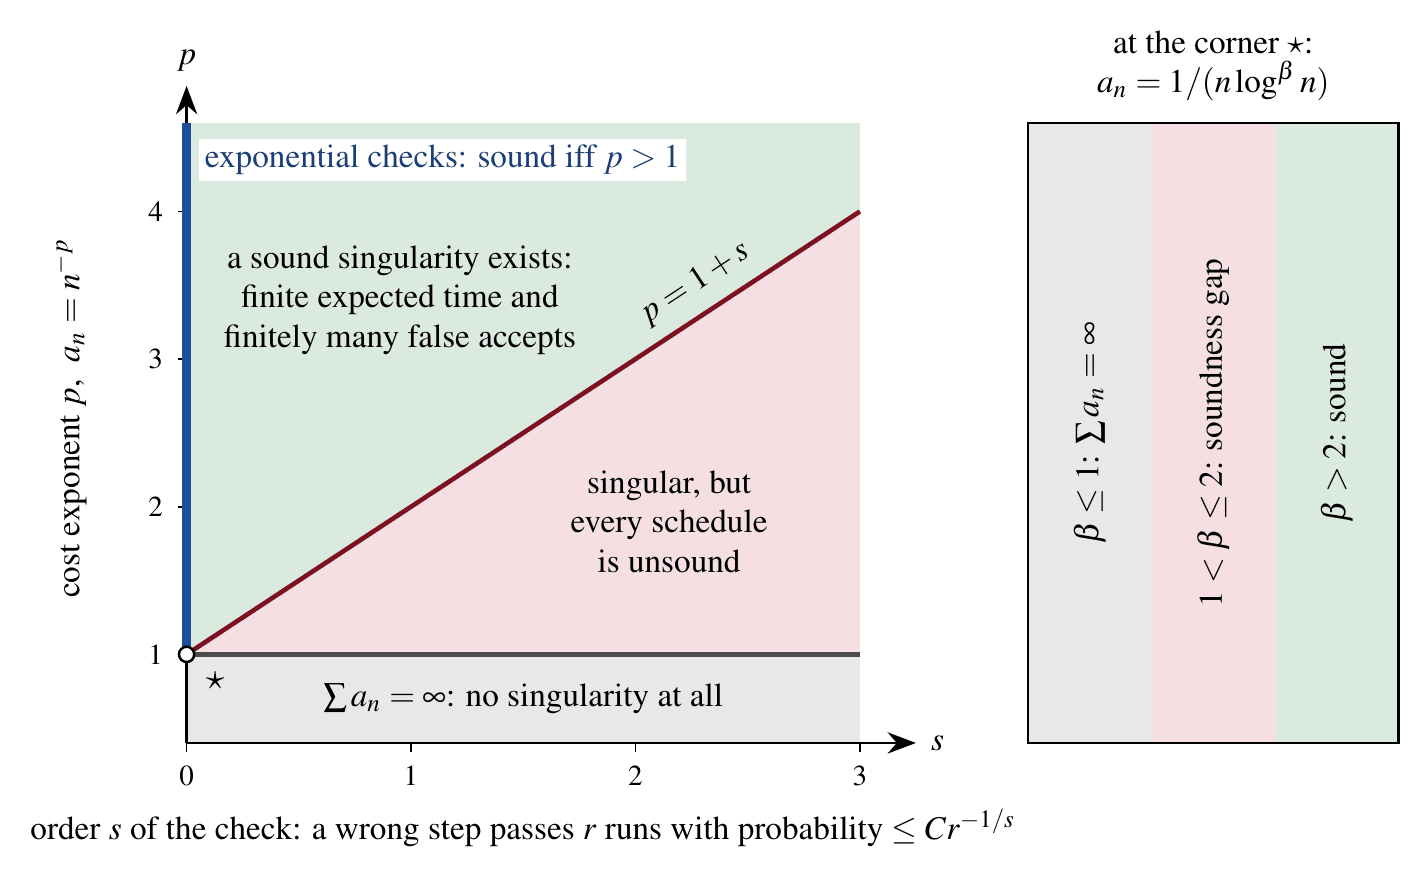
\includegraphics[width=0.86\textwidth]{figures/fig_regimes}
\caption{The phase diagram of Corollary~\ref{cor:phase} in the plane of the polynomial order $s$ of the checks and the exponent $p$ of the cost law $a_{n}=n^{-p}$. No singularity for $p\le1$; singular chains that are all unsound for $1<p\le1+s$; sound singular chains for $p>1+s$. The axis $s=0$ is the case of exponential checks, sound for every $p>1$. The panel at the corner refines the line $p=1$ by the logarithmic family $a_{n}=1/(n\log^{\beta}n)$ of Corollary~\ref{cor:gap}.}
\label{fig:regimes}
\end{figure*}
